%!TEX program = xelatex
\documentclass[10pt, compress]{beamer}
\usetheme[titleprogressbar]{m}

\usepackage{booktabs}
\usepackage[scale=2]{ccicons}
\usepackage{minted}
\usepackage{listings}
\usepackage{color}
\usepackage{hyperref}



\usepgfplotslibrary{dateplot}

\usemintedstyle{trac}

\title{\LARGE Tools for Time Series Analysis}
\subtitle{Optimized implementations in R}
\author{Student: Eduarda Tatiane Caetano Chagas\\ 
Teacher: Alejandro Cesar Frery Orgambide}
\institute{LaCCAN – Laboratório de análise e computação científica}

\begin{document}

\maketitle


\begin{frame}[fragile]
\frametitle{Work goals}
\begin{sloppypar}
\textit{\textbf{\Large "Implement time series analysis functions using Information Theory descriptors; Implement an interface to the application
Functions; Validate the interface and functions with end users."}}
\end{sloppypar}
\end{frame}

\begin{frame}[fragile]
\frametitle{Work goals}
\begin{sloppypar}
\textit{\textbf{\Large "\colorbox{gray}{Implement time series analysis functions} \colorbox{gray}{using Information Theory descriptors}; Implement an interface to the application
Functions; Validate the interface and functions with end users."}}
\end{sloppypar}
\end{frame}

\begin{frame}[fragile]
\frametitle{Time Series}
\begin{sloppypar}
\textit{\textbf{\Large "Time series are set of data obtained from an observational process over a determined period of time, not necessarily divided into equal spaces, being characterized by the serial dependence between observations."}}
\end{sloppypar}
\end{frame}

\begin{frame}[fragile]
\frametitle{Time Series}
\begin{sloppypar}
\textit{\textbf{\Large "Time series are \colorbox{gray}{set of data} obtained from an observational process over a determined period of time, not necessarily divided into equal spaces, being characterized by the serial dependence between observations."}}
\end{sloppypar}
\end{frame}

\begin{frame}[fragile]
\frametitle{Time Series}
\begin{sloppypar}
\textit{\textbf{\Large "Time series are \colorbox{gray}{set of data} obtained from an observational process over a determined period of time, not necessarily divided into equal spaces, being characterized by the \colorbox{gray}{serial dependence} between observations."}}
\end{sloppypar}
\end{frame}

\begin{frame}[fragile]
\frametitle{Areas of expertise}
\begin{figure}
  \centering
   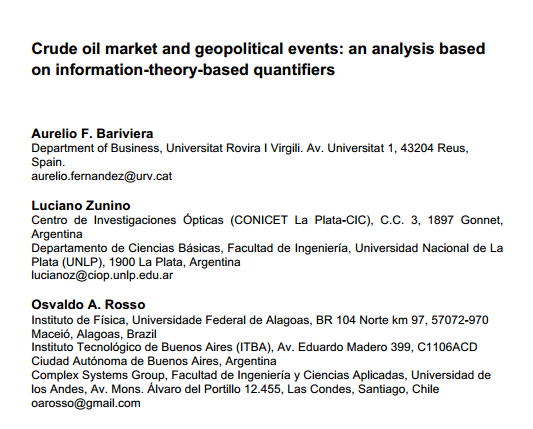
\includegraphics[width=10cm,height=7cm]{CrudeOil.png}
\end{figure}
\end{frame}

\begin{frame}[fragile]
\frametitle{Areas of expertise}
\begin{figure}
  \centering
   
\includegraphics[width=10cm,height=7cm]{StockMarket.png}
\end{figure}
\end{frame}

\begin{frame}[fragile]
\frametitle{Areas of expertise}

\begin{figure}
  \centering
   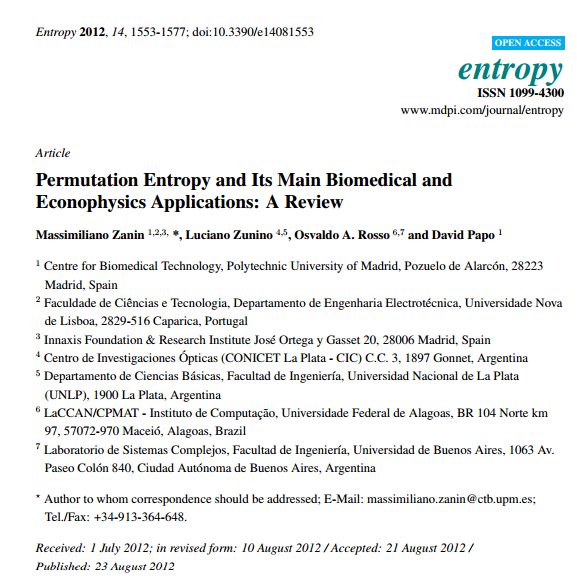
\includegraphics[width=8cm,height=6cm]{Biomedical.png}
\end{figure}
\end{frame}

\begin{frame}[fragile]
\frametitle{Tools present}

\begin{figure}
  \centering
   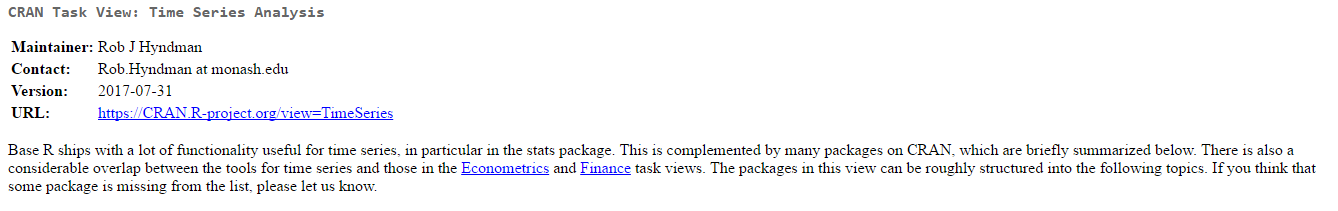
\includegraphics[width=11cm,height=3cm]{CRAN.png}
\end{figure}
\end{frame}

\begin{frame}[fragile]
\frametitle{Tools present}

\begin{figure}
  \centering
   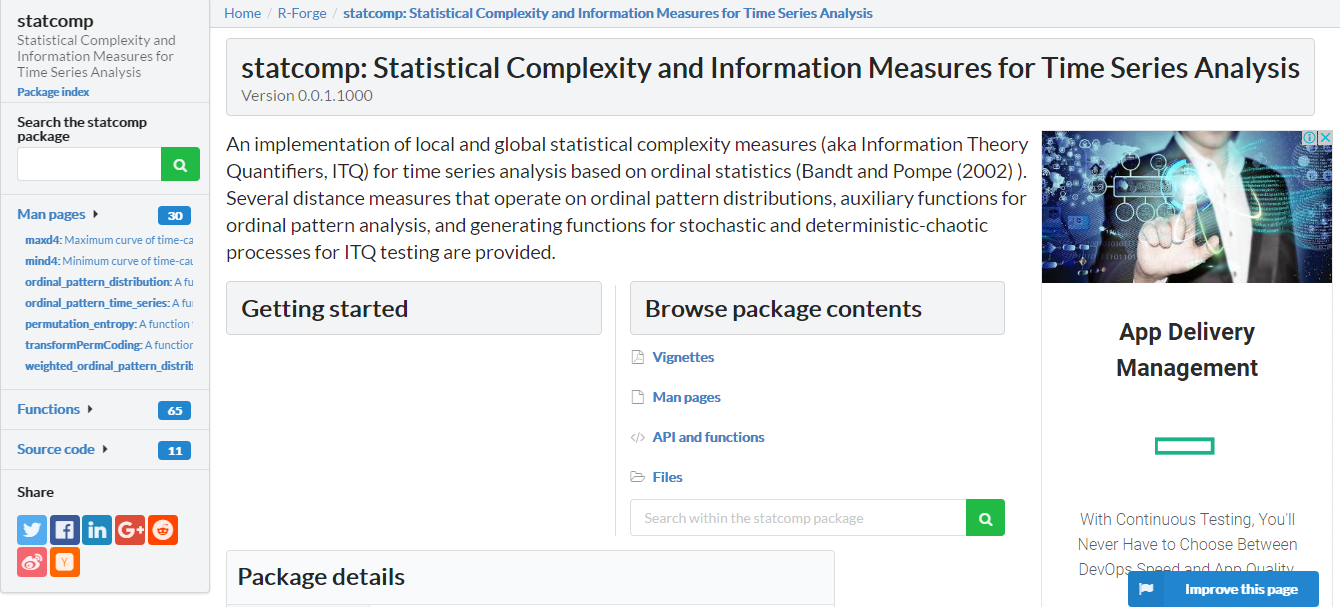
\includegraphics[width=10cm,height=7cm]{statcomp.png}
\end{figure}
\end{frame}

\begin{frame}[fragile]
\frametitle{Goals}
 
\textbf{\Large Researchers' main needs:}\\

-\textit{Friendly graphical tool;}

-\textit{Features
Fast, efficient and numerically reliable;} 

-\textit{Portability for several
operating systems and hardware architectures;}

-\textit{Use of FLOSS tools.} 

\end{frame}

\begin{frame}[fragile]
\frametitle{Methodology}

\begin{figure}
  \centering
   
\includegraphics[width=10cm,height=5cm]{ferramentas.png}
\end{figure}

\end{frame}


\begin{frame}[fragile]
\frametitle{Methodology}
 
\textbf{\Large Stages of the analysis process}\\

\textbf{Symbolization}

-\textit{Process of symbolization of Bandt and Pompe}\\

\textbf{Extraction of information}

-\textit{Entropy} 

-\textit{Stochastic distances}

-\textit{Statistical complexity} 

\end{frame}

\begin{frame}[fragile]
\frametitle{Symbolization of Bandt and Pompe}

\begin{figure}
  \centering
   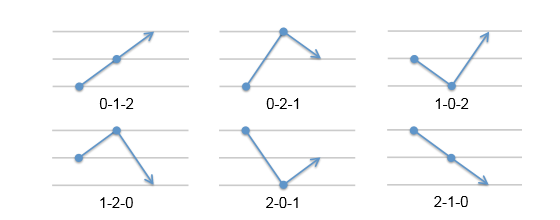
\includegraphics[width=10cm,height=6cm]{p.png}
\end{figure}
\end{frame}


\begin{frame}[fragile]
\frametitle{Histogram}

\begin{figure}
  \centering
   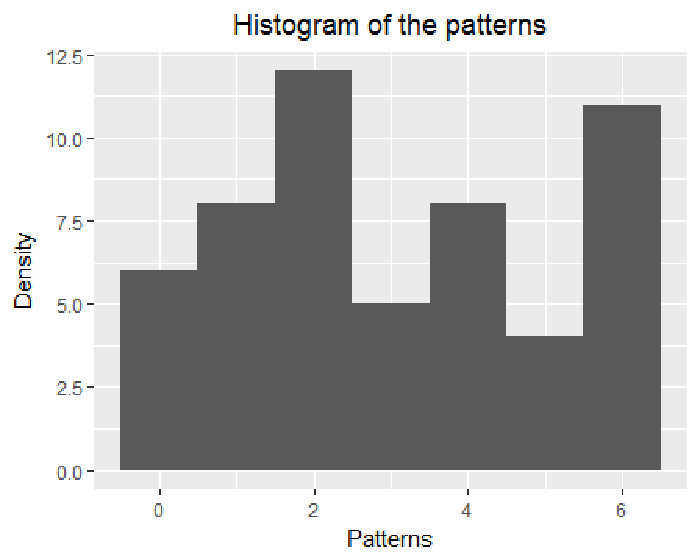
\includegraphics[width=8cm,height=6cm]{Rplot02.pdf}
\end{figure}
\end{frame}

\begin{frame}[fragile]
\frametitle{Entropy}

- Corresponds to the quantitative measure of uncertainty of a structure described by a probability distribution.

\end{frame}

\begin{frame}[fragile]
\frametitle{Shannon's Entropy}

- Be like that, $h=(h_1,\dots,h_{N!})$ the histogram of proportions of $N!$ patterns observed from the time series $x$.

- We calculate the Shannon entropy:

\begin{equation}
 H(h) = \sum_{i=1}^{N!} (-\log h_i) h_i ,
\label{eq:Entropia}
\end{equation}

\end{frame}
 
\begin{frame}[fragile]
\frametitle{Stochastic distance}

- By measuring the similarity between two time series, this measure is calculated by analyzing their respective probability distributions.

\end{frame}

\begin{frame}[fragile]
\frametitle{Stochastic distance}

- We then calculate the distance from Jensen-Shannon to the uniform distribution $ u=(1/N!,\dots,1/N!)$.

\begin{equation}
D( h, u) = \sum_{i=1}^{N!} \Big(h_i \log\frac{h_i}{u_i} +
u_i \log\frac{u_i}{p_i}
\Big),
\end{equation}

wherein $u_i=1/N!$.
\end{frame}

\begin{frame}[fragile]
\frametitle{Stochastic distance}
 \begin{lstlisting}
euclidian_distance<-function(probability){
  c = rep(1/length(probability),length(probability))
  distance = sum((probability-c)^2)
  return(sqrt(distance))
}
euclidian_quadratica_distance<-function(probability){
  c = rep(1/length(probability),length(probability))
  distance = sum((probability-c)^2)
  return(distance)
}
manhattan_distance<-function(probability){
  c = rep(1/length(probability),length(probability))
  distance = sum(abs(probability-c))
  return(distance)
}
\end{lstlisting}
\end{frame}


\begin{frame}[fragile]
\frametitle{Stochastic distance}
 \begin{lstlisting}
kullback_leibler_divergence<-function(probability){
  c = rep(1/length(probability),length(probability))
  distance <- probability * log(probability/c)
  distance[is.nan(distance)] <- 0
  return(sum(distance))
}
\end{lstlisting}
\end{frame}

\begin{frame}[fragile]
\frametitle{Stochastic distance}
 \begin{lstlisting}
hellinger_Distance<-function(probability){
  c = rep(1/length(probability),length(probability))
  distance = sum((sqrt(probability)-sqrt(c))^2)*0.5
  return(sqrt(distance))
}

jensenDivergence<-function(p){
  q = rep(1/length(p),length(p))
  s_p = shannonEntropy(p)
  s_q = shannonEntropy(q)
  s_pq = shannonEntropy((p+q)/2)
  divergence = sum( s_pq - (s_p/2) - (s_q/2))
  return(divergence)
}
\end{lstlisting}
\end{frame}

\begin{frame}[fragile]
\frametitle{Stochastic distance}
 \begin{lstlisting}
wootters_distance<-function(probability,q){
  c = rep(1/length(probability),length(probability))
  dis = sum(sqrt(probability*c))
  dis = acos(dis)
  return(dis)
}
chebyshev_distance<-function(probability){
  c = rep(1/length(probability),length(probability))
  L = abs(probability - c)
  return(max(L))
}
\end{lstlisting}
\end{frame}

 
\begin{frame}[fragile]
\frametitle{Statistical complexity}

- Seek to find interaction structures
Of dependency between the elements of a given series.

\end{frame}
 
\begin{frame}[fragile]
\frametitle{Statistical complexity}

- We calculate the second descriptor of our time series: its Statistical Complexity:

\begin{equation}
C( h, u) = H( h) D( h,  u).
\end{equation}

\end{frame}

\begin{frame}[fragile]
\frametitle{Statistical complexity Plane}

- Each time series can then be described by a point $(H( h), C( h,  u))$.
The set of all pairs $(H( h), C( h,  u))$ for anytime series described by length standards $N$ meet in a compact subassembly $ R^2$: The Statistical complexity Plane.

\end{frame}

\begin{frame}[fragile]
\frametitle{Statistical complexity Plane}

\begin{figure}
  \centering
   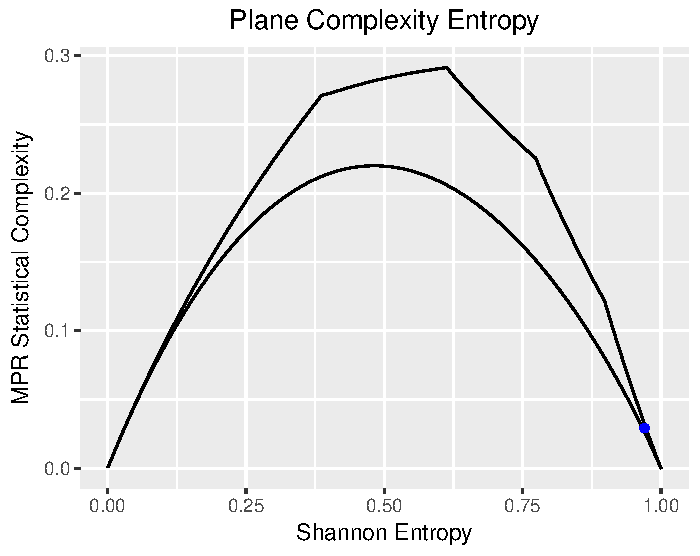
\includegraphics[width=8cm,height=6cm]{Rplot3.pdf}
\end{figure}
\end{frame}

\begin{frame}[fragile]
\frametitle{Time Series}

\begin{figure}
  \centering
   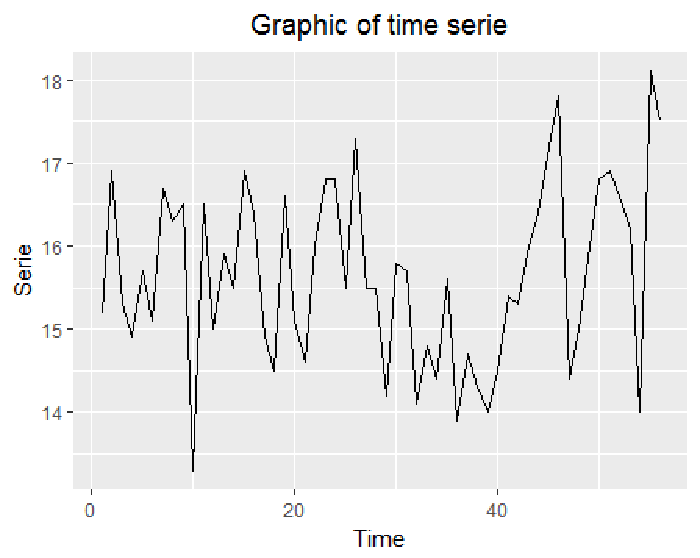
\includegraphics[width=8cm,height=6cm]{Rplot.pdf}
\end{figure}
\end{frame}

\begin{frame}[fragile]
\frametitle{Time Series and the patterns}

\begin{figure}
  \centering
   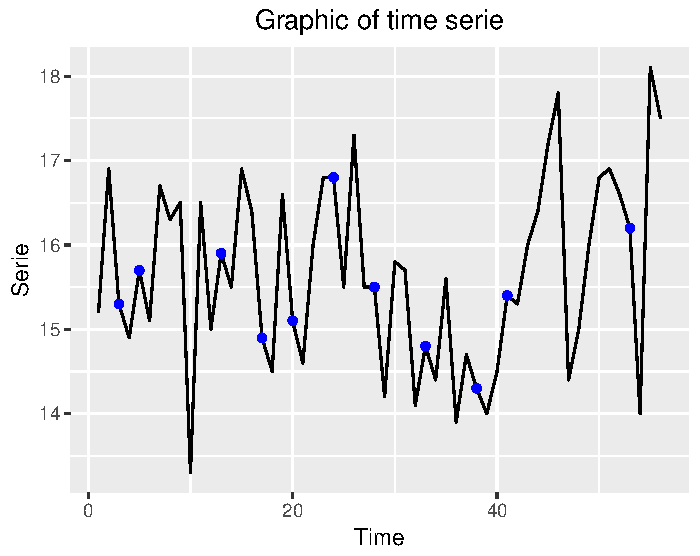
\includegraphics[width=8cm,height=6cm]{Rplot04.pdf}
\end{figure}
\end{frame}

\begin{frame}[fragile]
\frametitle{Data Mining}

- They have the characteristic of substantially reducing the size of the data, while maintaining its main characteristics intact.
\end{frame}

\begin{frame}[fragile]
\frametitle{Piecewise Aggregate Approximation}
\begin{figure}
  \centering
   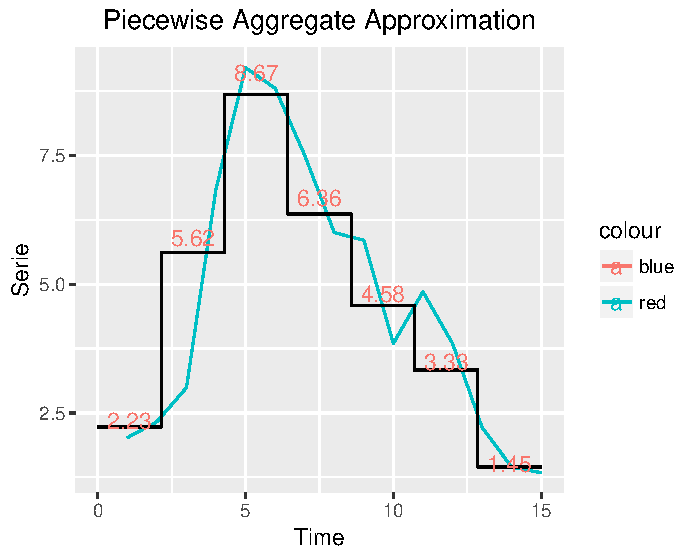
\includegraphics[width=10cm,height=6cm]{PAA.pdf}
\end{figure}
\end{frame}

\begin{frame}[fragile]
\frametitle{Perceptually Important Points}
\begin{figure}
  \centering
   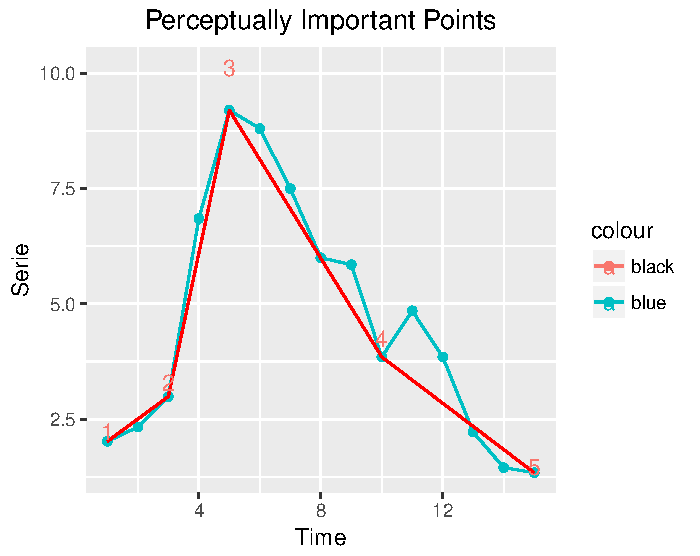
\includegraphics[width=10cm,height=6cm]{PIP.pdf}
\end{figure}
\end{frame}

\begin{frame}[fragile]
\frametitle{Symbolic Aggregate Approximation}
\begin{figure}
  \centering
   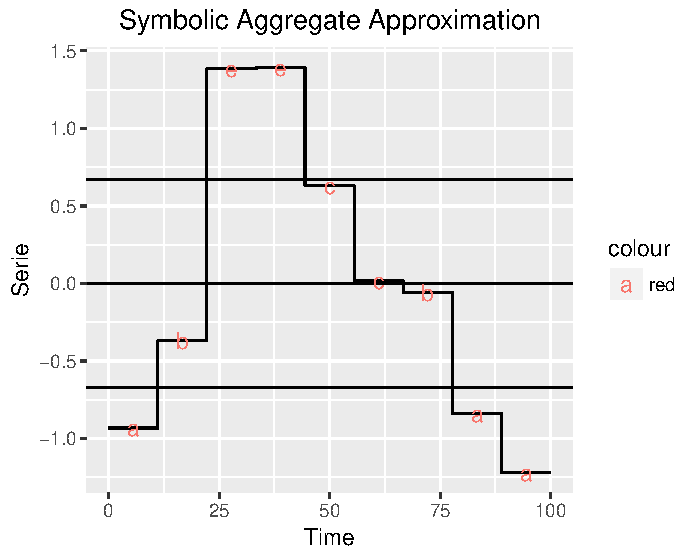
\includegraphics[width=10cm,height=6cm]{SAX.pdf}
\end{figure}
\end{frame}

\begin{frame}[fragile]
\frametitle{System}

- The system was designed and developed in a modular way, consisting of the following units:

\begin{itemize}
\item Symbolization module;
\item Analysis module;
\item Visualization and interaction module;
\end{itemize} 

\end{frame}

\begin{frame}[fragile]
\frametitle{System}

- To increase the applicability of the system, it is possible to both generate series and read data in various formats (TXT, CSV or XLSX), and the following user chooses:

\begin{itemize}
\item Generate series graph;
\item Calculate various types of Entropy;
\item Calculate various types of Stochastic Distances;
\item Calculate statistical complexities;
\item Generate Pattern Histogram;
\item Identify the characteristic point of the series in the Entropy-Complexity plane.
\end{itemize}

\end{frame}

\begin{frame}[fragile]
\frametitle{Work Goals}
\begin{sloppypar}
\textit{\textbf{\Large "Implement time series analysis functions using Information Theory descriptors; \colorbox{gray}{Implement an interface to the application}
\colorbox{gray}{functions}; Validate the interface and functions with end users."}}
\end{sloppypar}
\end{frame}

\begin{frame}[fragile]
\frametitle{Graphic interface}
\begin{figure}
  \centering
   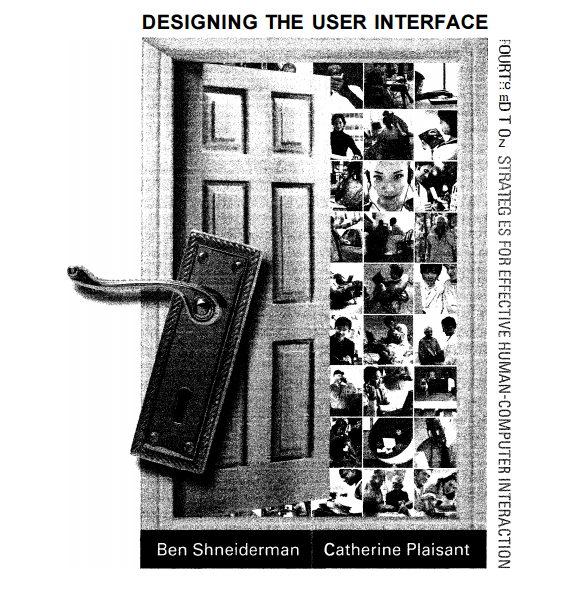
\includegraphics[width=6cm,height=6cm]{interface.png}
\end{figure}
\end{frame}

\begin{frame}[fragile]
\frametitle{Graphic interface}

-\textbf{ \Large Shneiderman Gold Rules:}

\begin{itemize}
\item Strive for consistency;
\item Meet universal usability;
\item Provide informative feedback;
\item Dialogues that indicate the end of an action;
\item Avoid mistakes;
\item Allow for easy stock reversal;
\item Support user control;
\item Reduce short-term memory load.
\end{itemize}
\end{frame}

\begin{frame}[fragile]
\frametitle{Graphic interface}
\begin{figure}
  \centering
   
\includegraphics[width=10cm,height=6cm]{FInterface.png}
\end{figure}
\end{frame}

\begin{frame}[fragile]
\frametitle{Graphic interface}
\begin{figure}
  \centering
   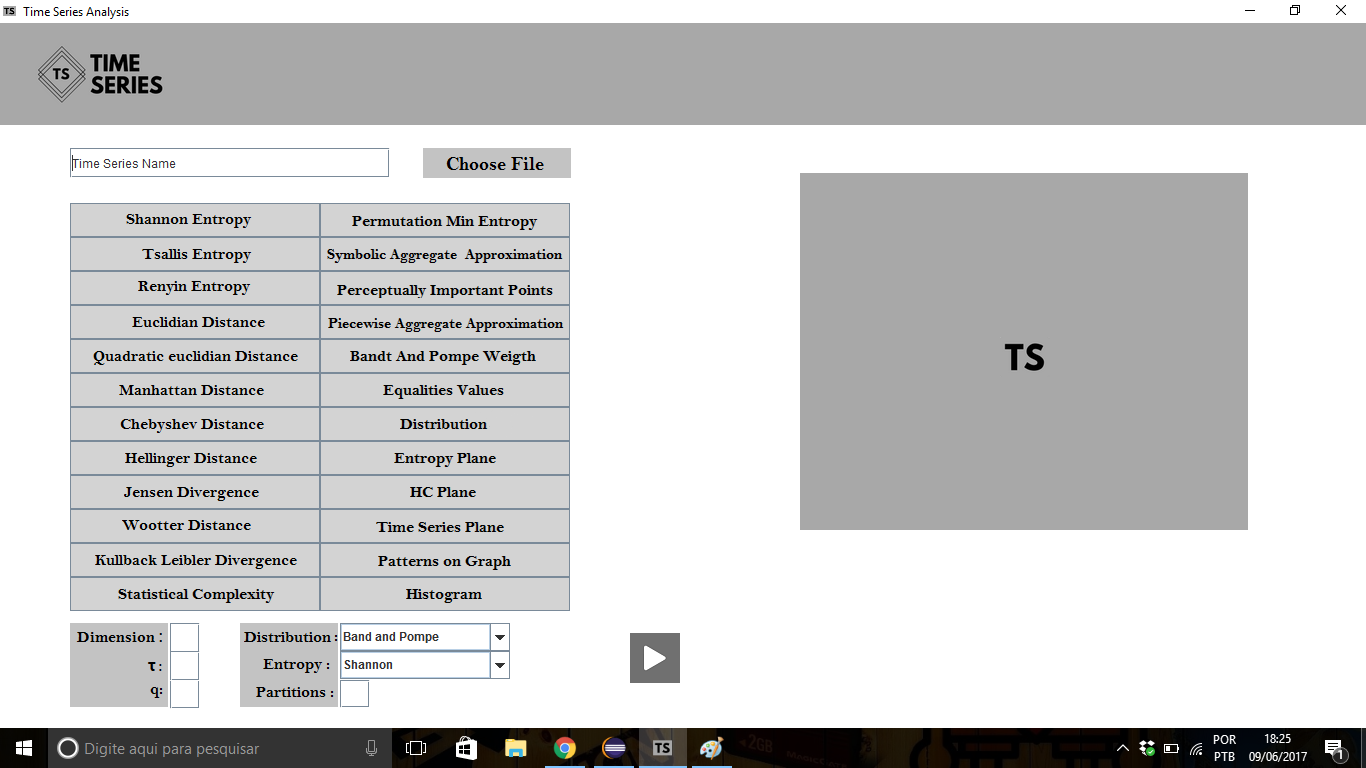
\includegraphics[width=10cm,height=6cm]{tela4.png}
\end{figure}
\end{frame}

\begin{frame}[fragile]
\frametitle{Graphic interface}
\begin{figure}
  \centering
   
\includegraphics[width=10cm,height=6cm]{rgtk2.png}
\end{figure}
\end{frame}

\begin{frame}[fragile]
\frametitle{Work Goals}

\textit{\textbf{\Large "Implement time series analysis functions using Information Theory descriptors; Implement an interface to the application functions; \colorbox{gray}{Validate the interface and functions} \colorbox{gray}{with end users.}"}}

\end{frame}

\begin{frame}[fragile]
  \frametitle{References}
\begin{itemize}

\item{Characterization of vehicle behavior with Information Theory / Aquino, A. L. L. et al. (2015)}

\item{A Mathematical Theory of Communication / Shannon, C. E. (1948)}

\item{Measures of statistical complexity: Why? / Feldman and Crutcheld (1998)}

\item{Permutation entropy: A natural complexity measure for time series / Bandt and Pompe (2002)}

\end{itemize}
\end{frame}

\plain{Dúvidas?}

\end{document}